\chapter{Introduction}

\epigraph{Me caí, me paré, caminé, me subí \\ me fui contra la corriente \\ y también me perdí}{Soy Yo \\ Bomba Estéreo, 2015}

\section{Context}

This thesis is the capstone project of my master's program, between the academic years 2019-2021 at MIT Media Lab, where I am a Research Assistant at the groups Opera of the Future and Future Sketches. The work presented here has been developed mostly while working remotely during the COVID19 pandemic, while at home in Boston MA.

This thesis is a collection of media arts instruments, using tiny \acrshort{ML}, and with a strong emphasis on \acrlong{AI} ethics and \acrlong{DIY}. Its main audience is beginners and artists, and it is my hope that this work can inspire a new generation of instrument makers, artists, designers, educators, programmers, policy makers, activists, and enthusiasts.

\acrfull{ML} has several barriers of entry, including cost, complexity, and difficulty. Since my practice is based on sharing and working on the open with different communities, I am not a fan of the current state of industrial \acrshort{ML} that relies on proprietary software and hardware. This tends to happen because their ML models are aiming for high precision, and need to be trained for long periods of time, using expensive non open computational resources, with huge datasets that often are scraped from the internet without the explicit consent of the people, and a byproduct of surveillance capitalism.

Since all \acrshort{ML} algorithms are written by humans, and then trained on biased data, and they are deployed to the world, where they affect our lives. These imperfections are highlighted over the course of this thesis, by being explicit about the assumptions and quantizations performed when working with data.



This thesis proposes a scaling down of \acrshort{ML}, to make it more accessible to artists, it is my belief that computational technology is 

A 

\cite{website-talk-technology-and-public-art-rafael-lozano-hemmer}
36m28s
Rafael Lozano-Hemmer: Face recognition needs to be banned in all applications except art.

TODO: add Zoom example of garbage speech to text


 in expensive or rented resources, such as the service Google Colab, which allows you to share and train ML models on the cloud. This thesis shows users how to build \acrshort{ML} art systems that can circumvent this and allow for more control of their data.

Artists have unprecedented access to new tools for making new tools and instruments, and this thesis intends to be a foundation for a new generation of instruments for manipulating audiovisual material, using \acrshort{ML}. This approach is really exciting because it allows beginners and artists to train their instruments instead of programming them, by inputting data for tuning, instead of having to write lines of code and fixed thresholds for changing their behavior.

In this first example, I said the following phrase "This is a text to show that Zoom transcription does not work with my voice, because of my accent."

\begin{figure}[ht]
  \centering
  
\includegraphics[width=0.75\linewidth,height=0.25\textheight,keepaspectratio]{images/zoom-introduction.jpg}
  \caption{Screen capture of speech to text on Zoom, introduction}
  \caption*{Screen capture by myself}
  \label{fig:zoom-voice}
\end{figure}

In this other example, I said out loud the names of my thesis commitee members: Tod Machover, Mitchel Resnick, Zach Lieberman.

\begin{figure}[ht]
  \centering
  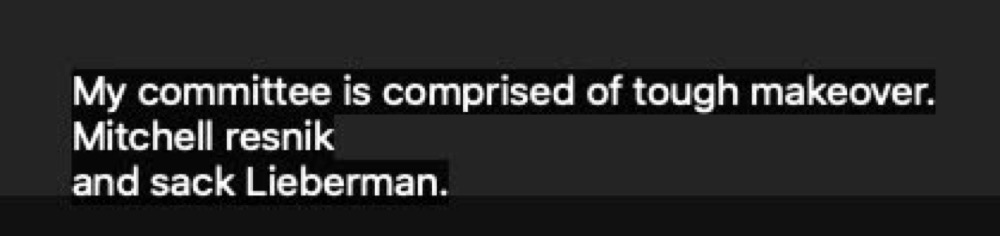
\includegraphics[width=0.75\linewidth,height=0.25\textheight,keepaspectratio]{images/zoom-commitee.jpg}
  \caption{monome norns}
  \caption*{Screen capture of speech to text on Zoom, introduction}
  \label{fig:zoom-committee}
\end{figure}

My guess is that these errors come from a combination of factors, including my English accent, and the Chilean accent not being widely included on the databases used for training.

Years ago I decided against using text completion (if you have ever interacted with me over text, I typed every single character :)), and also I don't use any voice assistants, including Apple's Siri, Amazon's Alexa,  Google's Google Assistant, or Microsoft's Cortana.

\begin{figure}[ht]
  \centering
  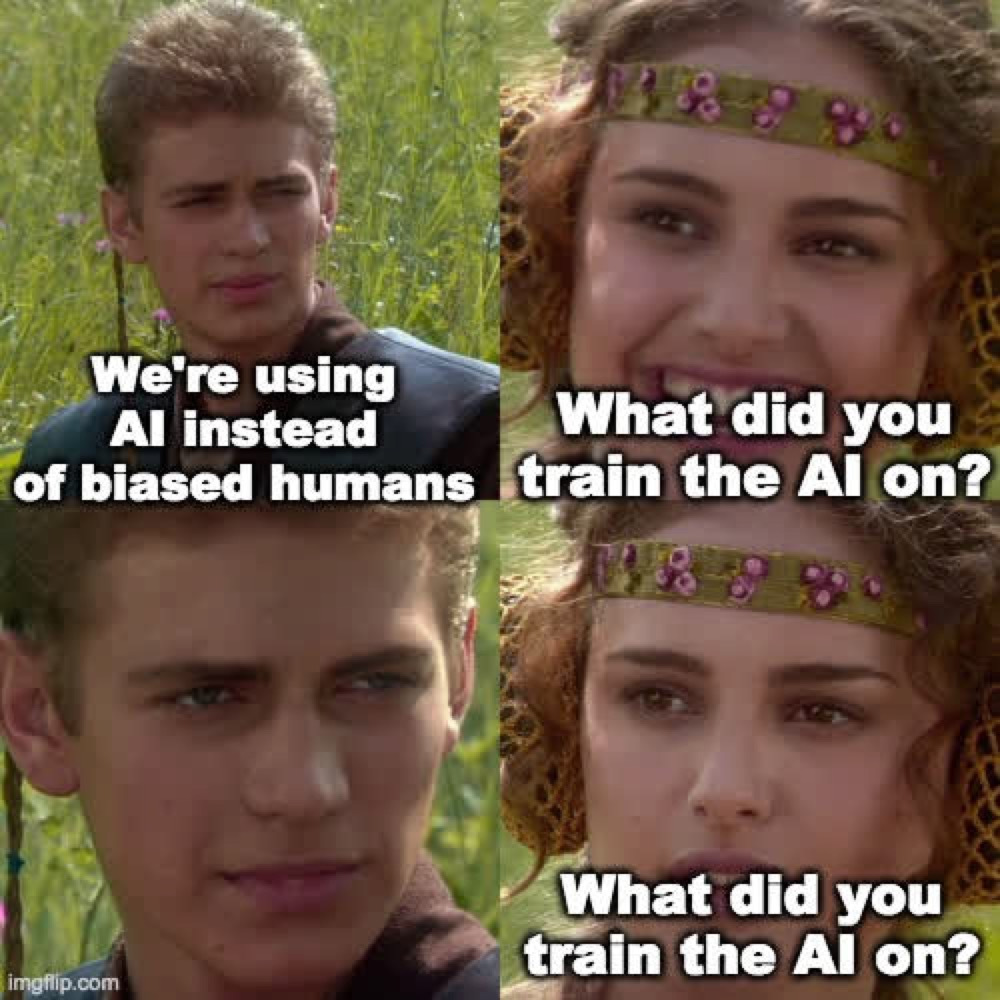
\includegraphics[width=0.75\linewidth,height=0.25\textheight,keepaspectratio]{images/meme-star-wars.jpg}
  \caption{Meme about biased data}
  \caption*{Retrieved from \cite{website-twitter-janellecshane-meme}}
  \label{fig:meme-star-wars}
\end{figure}

\begin{figure}[ht]
  \centering
  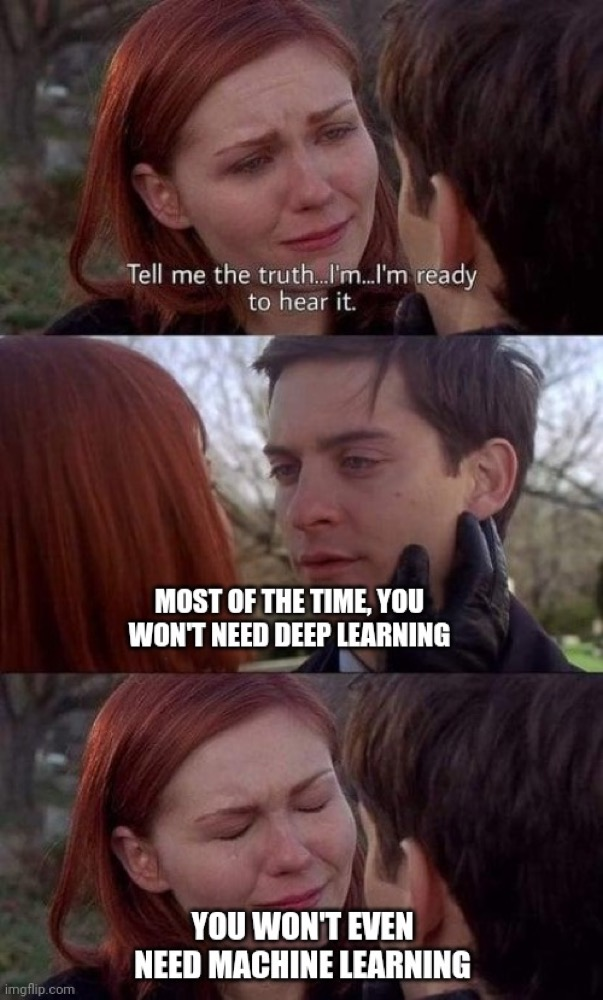
\includegraphics[width=0.75\linewidth,height=0.25\textheight,keepaspectratio]{images/meme-spider-man.jpg}
  \caption{Meme about biased data}
  \caption*{Retrieved from \cite{website-twitter-dynamicwebpaige-meme}}
  \label{fig:meme-spider-man}
\end{figure}

TODO: Add an example of a biased dataset that is commonly used.

The proliferation of surveillance tools and now of microcontrollers allows for an even more pervasive surveillance and data leaks by governments and corporations. This thesis allows for beginners and artists to develop their own databases, by self sensing and surveillance. TODO: explain self-sensing and surveillance, and explain harms of surveillance, with an example.

Low power and repurposable
Tiny \acrshort{ML} is defined as \acrshort{ML} performed with low-power devices TODO: add citation or mention that it is my own definition. The proposal of media arts instruments that can run on little power, rechargeable batteries is a friendly use of resources for experimentation in arts. This is in contrast with the high power use and critique of other emerging fields such as Non Fungible Tokens (NFTs) and cryptoart. The proposal of these scriptable open source instruments allows for users to continuously tweak and modify their instruments, repurpose the hardware, and enable sharing.

TODO: Add a reference to an early tiny ML paper.

\section{Objectives}

With the release of TensorFlow Lite Micro, the TinyML Foundation, new avenues have been opened for creative expression using \acrshort{ML} in microcontrollers.

TensorFlow is a library by Google for \acrshort{ML}. They have released different flavors for different devices, including TensorFlow.js for working with KavaScript and in the browser, and TensorFlow Lite for devices with less memory, like mobile devices. The newer TensorFlow Lite Micro is even lighter and intended for working on microcontrollers, and that is the flavor I am using in this thesis.

in a paragraph here that combines the points you make in the first paragraphs -> the main contributions of YOUR thesis... which it seems is basically just addressing a bunch of the context section? Blakeley Payne's thesis does a good job of outlining contributions. It's also good to do here to understand where you are going

Homebrew examples, teach people how to build their own databases, and how to circumvent corporations view.

TODO: Terms and conditions comic book. If people were to read terms and conditions, it would take them X years

You can train an instrument to only detect your voice, your accent, your living conditions.

TODO: add blurb main inspiration about trail building and skatepark, and playpens, sandbox

TODO: Raspberry Pi example, it’s cheap but it needs a lot of extra hardware to be used

Navigating legal documents can be hard. In 2010, GameStation added a soul clause to their terms of conditions as an April Fool's prank, making them legal owners of thousands of customers' souls \cite{website-huffpost-gamestation-soul-clause}.



TODO: Terms and conditions citation: (copied this in from my thesis, but check out McDonald and Cranor 2008) https://kb.osu.edu/handle/1811/72839 "Just considering privacy policies shown to people online in one year, it's been estimated that consumers would need approximately 244 hours to read, not skim, privacy policies shown to them in one calendar year."

\section{Thesis outline}

This thesis has cover the following chapters:

\begin{enumerate}
  \item Chapter 1, Introduction: the context and summary of this thesis.
  \item Chapter 2, Tiny trainable instruments: description of the design strategies for the software and hardware, description of the support team working on this thesis.
  \item Chapter 3, Early experiments: my earlier work that led to this thesis, in the topics of media arts education, microcontrollers, and \acrshort{ML}, among others.
  \item Chapter 4, Background and inspiration: work by other people which has informed my work.
  \item Chapter 5, Project evaluation: user feedback, field notes.
  \item Chapter 6, Conclusions and future work: next iterations of the instruments, and their proposed use for educators and artists.
  \end{enumerate}
